\chapter{Experiments with Deep Domain Adaptation on Spectral Data}
\label{exp_chapter}

In previous chapters, we have selected suitable astronomical data
and surveyed and choosen suitable deep domain adaptaion methods.
Now, we carry out experiments with the selected methods
on astronomical spectra from the SDSS and LAMOST spectroscopic sky surveys.

Firstly, we create source and target datasets for experiments.
Then, we reduce the data to two-dimensions
so we are able to visualise the data
and investigate distributions of both the source and target data.
% TODO CNN abbreviation
Thirdly, we introude a CNN baseline model
which serves as benchmark for comparison of deep domain adapation methods.
Finally, we employ five deep domain adaptation methods
and evaluate the adapted results to see 
if astronomical spectroscopy can benefit from deep domain adaptation.

\section{Data Preparation}

% TODO introduction to section

Our data of source domain consists of 4\,851\,200 optical spectra from the SDSS DR14 catalog
and the corresponding SDSS DR14Q catalog of 649\,791 spectra of 526\,356 QSO objects
(we have to distinguish an object and a spectrum
because each astronomical object could be observed multiple times
having more spectra).
Both catalogs are introduced in~Subsection~\ref{sdss}.
However, 20\,279 spectra of QSOs cannot be idenfified
% TODO describe the bug in SDSS DR14Q catalog
because there is a bug in the SDSS DR14Q catalog.
Therefore, we are able to identify only 629\,512 spectra of all QSOs.
% TODO describe that spectra are stored in individual FITS
% TODO spectra are downloaded according to SDSS DR14 catalog
% TODO lite versions extracted COADD
Next, we need to cross-match the SDSS DR14 and DR14Q catalogs
to merge the data stored in individual FITS files with QSO labels.
The cross-matching is based on triplet of
\textit{plate number}, \textit{Modified Julian Date of obesrvation} and \textit{fiber number} that is unique to each spectrum.
Additionally to the 20\,279 spectra of QSOs lost due to the bug in the DR14Q catalog,
we were unable to cross-match 55 QSOs with the SDSS DR14 catalog.
Therefore, totally we have 629\,457 spectra of QSOs
for which we have actual data in FITS files and not only metadata in catalogs.

Complement to the source domain in domain adapation is the target domain.
We selected data from LAMOST DR5 to be target domain data
for reasons described in Subsection~\ref{lamost}.
The LAMOST DR5 general catalog contains 9\,026\,365 spectra
and the most complete catalog of QSOs has 42\,552 spectra.
Again, we cross-matched the LAMOST DR5 catalog and the catalog of QSOs
according to quartet of \textit{plan identifier}, \textit{local Modified Julian Date} (one less the Modified Julian Date), \textit{spectrograph identifier} and \textit{identifier of fiber}.
We were able to cross-match 31\,755 spectra of QSOs with the general catalog
effectively losing 10\,797 spectra of QSOs.
We believe that LAMOST has good reasons for not including those spectra in the LAMOST DR5 catalog.

However, the labels of QSOs from LAMOST are incompatible with labels from SDSS
because the criteria of what is a QSO are different in SDSS and LAMOST
(see Section~\ref{large_spec_surveys}).
For us the ground truth are labels of SDSS DR14Q catalog
while the labels of LAMOST serves only for evaluation purposes
not for training.
% TODO infer impact of performace measurement
Therefore, there might be spectra truly QSOs in LAMOST
not yet identified by LAMOST cripling our performance measurement
that will be biased.

Having assigned labels of QSOs to individual spectra,
% TODO footnote what is FITS file?
we need to extract the spectra from individual FITS files
because learning of neural networks requires datasets to be in form of design matrices.
A design matrix contains a different example (a spectrum) in each row
whereas each column of the design matrix corresponds to a different feature
(a measurement of flux in a specific wavelength).~\cite{goodfellow2016}

Fortunately, SDSS and LAMOST spectra have common wavelength grid in logarithmic wavelengths evenly space by 0.0001.
Although all spectra have a common wavelength grid,
the minimal and maximal wavelengths are different for each spectrum.
The Figure~\ref{wavemin_wavemax_hist} displays histograms of minimal and maximal wavelengths of all LAMOST spectra.
In this work, we aim to find QSOs in the LAMOST DR5.
Therefore, we would like to keep as many spectra as possible from the LAMOST~DR5.
To keep all spectra from the LAMOST~DR5,
we have to select wavelength range starting at 3\,839.7244~\AA{} (3.5843 in logarithmic wavelength)
which is the maximum from minimal wavelengths
and ending at 8\,914.597~\AA{} (3.9501 in logarithmic wavelength)
which is the minimum from maximal wavelengths.
The selection gives us a wavelength grid of 3659 logarithmically-spaced wavelengths
(each spectrum is a real vector of~\(\mathbb{R}^{3659}\)).

\begin{figure}
	\includegraphics[width=\textwidth]{img/wavemin_wavemax_hist.pdf}
	\caption{Minimal and maximal wavelengths of all LAMOST spectra.}
	\label{wavemin_wavemax_hist}
\end{figure}

Given the selected grid of wavelength we will lose some SDSS spectra
because not all of them have all mesurement in the range.
Figure~\ref{waves_cumulative_hist} shows cumulative histogram of how many spectra we will keep for cuts in different wavelengths.
We see that major drop are behind the selected minimal and maximal wavelengths
that means we will keep most of the spectra.
Precisely, the cut will drop 34\,487 spectra from our source dataset
including 1\,949 spectra of QSO.
Therefore, the source dataset has 4\,816\,713 spectra with 627\,508 spectra of QSOs that can enter a learing of a neural network.

\begin{figure}
	\includegraphics[width=\textwidth]{img/waves_cumulative_hist.pdf}
	% TODO captions of all figures and tables
	\caption{Cutting SDSS specta.}
	\label{waves_cumulative_hist}
\end{figure}

The original sizes of data are unnecessary for experimenting with deep domain adataption on astronomical spectra.
We store each spectrum as a vector of 3\,659 single-precision floating-point number (4 bytes).
The storage setting gives that the SDSS source dataset has about 70.5~GB
and the LAMOST target dataset 132.1~GB.
Data of such size usually cannot fit into memory
and access to a disk significantly slows learning on a GPU.

Therefore, we have subsampled the data to the size of ImageNet~\cite{russakovsky2015}.
We believe that the size of ImageNet is more than reasonable
because ImageNet is the dataset
that enable the superiority of deep neural network in computer vision.
ImageNet has 1 million training examples, 50 thousand validation examples
and 100 thousand testing examples.
Accordingly, we randomly subsampled of source and target datasets
obtaining training sets of size 1 million
and validation sets of size 50 thousand
while the rest of the data serves as testing sets.
We summarise sizes of datasets with corresponding number of QSOs in Table~\ref{datasets_sizes}.
Table~\ref{datasets_sizes} shows a significant class imbalance in the LAMOST DR5
where QSOs are very rare (less then 0.4\%).

\begin{table}
	\begin{center}
	\begin{tabular}{|l|r|r|}
		\hline
		Name & QSOs & Total spectra \\ \hline \hline
		SDSS DR14 & 629\,457 (12.98\%) & 4\,851\,200 \\ \hline
		usable SDSS DR14 & 627\,508 (13.03\%) & 4\,816\,713 \\ \hline
		SDSS training set & 130\,904 (13.09\%) & 1\,000\,000 \\ \hline
		SDSS validation set & 6\,552 (13.10\%) & 50\,000 \\ \hline
		LAMOST DR5 v3 & 31\,755 (0.35\%) & 9\,026\,365 \\ \hline
		LAMOST training set & 3\,517 (0.35\%) & 1\,000\,000 \\ \hline
		LAMOST validation set & 190 (0.38\%) & 50\,000 \\ \hline
	\end{tabular}
	\end{center}
	\caption{Sizes of datasets.}
	\label{datasets_sizes}
\end{table}

The last step of data preparation is min-max scaling of each spectrum into the \([-1; 1]\) range:

\begin{equation}
	\mathbf{x}_i = 2 \frac{\mathbf{x}_i - \min(\mathbf{x}_i)}{
		\max(\mathbf{x}_i) - \min(\mathbf{x}_i)} - 1,
\end{equation}

where \(\mathbf{x}_i \in \mathbb{R}^{3659}\) is a spectrum as defined in Chapter~\ref{da_chapter}
and functions \(\min(\cdot)\) and \(\max(\cdot)\) returns the smallest and the largest element of a given vectore respectively.

There are two benefits of the min-max scaling.
Firstly, the data will be in a suitable range for learning of neural networks
which will stabilise learning.
Secondly, the scaling will remove intensity properties of spectra
leaving us only with the spectrum shape which we are interesting in.

\section{Dimensionality Reduction}

PCA (Principal Component Analysis), 
t-SNE (t-Distributed Stochastic Neighbor Embedding)
and UMAP (Uniform Manifold Approximation and Projection).

\section{Baseline: Results without Use of Deep DA}

LeNet-5 and DeCAF.

\begin{figure}
	\includegraphics[width=\textwidth]{img/lenet_losses.pdf}
	\caption{Losses of LeNet-5}
	\label{lenet_losses}
\end{figure}

\tikzstyle{layer} = [align=center,draw=black,font=\tiny,rectangle,text centered]
\begin{figure}
\begin{center}
\subfloat[][LeNet-5]{
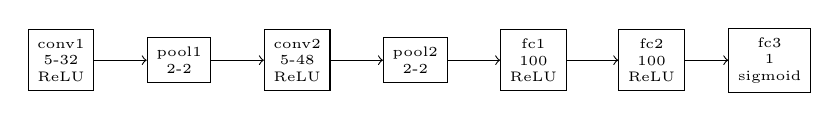
\begin{tikzpicture}[node distance=1.5cm]
	\node (conv1) [layer] {conv1\\5-32\\ReLU};
	\node (pool1) [layer,right of=conv1] {pool1\\2-2};
	\node (conv2) [layer,right of=pool1] {conv2\\5-48\\ReLU};
	\node (pool2) [layer,right of=conv2] {pool2\\2-2};
	\node (fc1) [layer,right of=pool2] {fc1\\100\\ReLU};
	\node (fc2) [layer,right of=fc1] {fc2\\100\\ReLU};
	\node (fc3) [layer,right of=fc2] {fc3\\1\\sigmoid};
	\draw [->] (conv1) -- (pool1);
	\draw [->] (pool1) -- (conv2);
	\draw [->] (conv2) -- (pool2);
	\draw [->] (pool2) -- (fc1);
	\draw [->] (fc1) -- (fc2);
	\draw [->] (fc2) -- (fc3);
\end{tikzpicture}
}\\
\subfloat[][DDC]{
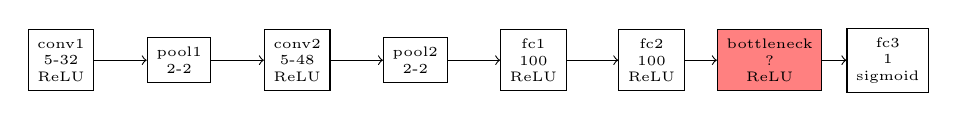
\begin{tikzpicture}[node distance=1.5cm]
	\node (conv1) [layer] {conv1\\5-32\\ReLU};
	\node (pool1) [layer,right of=conv1] {pool1\\2-2};
	\node (conv2) [layer,right of=pool1] {conv2\\5-48\\ReLU};
	\node (pool2) [layer,right of=conv2] {pool2\\2-2};
	\node (fc1) [layer,right of=pool2] {fc1\\100\\ReLU};
	\node (fc2) [layer,right of=fc1] {fc2\\100\\ReLU};
	\node (bottleneck) [layer,right of=fc2,fill=red!50] {bottleneck\\?\\ReLU};
	\node (fc3) [layer,right of=bottleneck] {fc3\\1\\sigmoid};
	\draw [->] (conv1) -- (pool1);
	\draw [->] (pool1) -- (conv2);
	\draw [->] (conv2) -- (pool2);
	\draw [->] (pool2) -- (fc1);
	\draw [->] (fc1) -- (fc2);
	\draw [->] (fc2) -- (bottleneck);
	\draw [->] (bottleneck) -- (fc3);
\end{tikzpicture}
}\\
\subfloat[][DANN]{
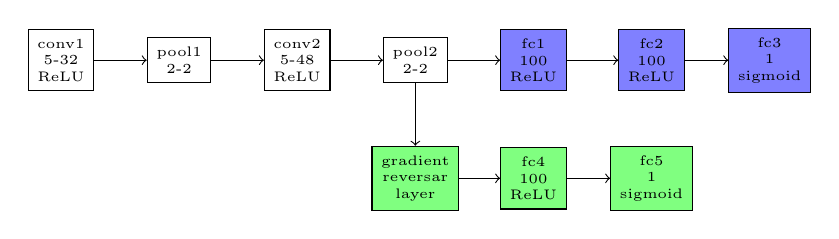
\begin{tikzpicture}[node distance=1.5cm]
	\node (conv1) [layer] {conv1\\5-32\\ReLU};
	\node (pool1) [layer,right of=conv1] {pool1\\2-2};
	\node (conv2) [layer,right of=pool1] {conv2\\5-48\\ReLU};
	\node (pool2) [layer,right of=conv2] {pool2\\2-2};
	\node (fc1) [layer,right of=pool2,fill=blue!50] {fc1\\100\\ReLU};
	\node (fc2) [layer,right of=fc1,fill=blue!50] {fc2\\100\\ReLU};
	\node (fc3) [layer,right of=fc2,fill=blue!50] {fc3\\1\\sigmoid};
	\node (grl) [layer,below of=pool2,fill=green!50] {gradient\\reversar\\layer};
	\node (fc4) [layer,right of=grl,fill=green!50] {fc4\\100\\ReLU};
	\node (fc5) [layer,right of=fc4,fill=green!50] {fc5\\1\\sigmoid};
	\draw [->] (conv1) -- (pool1);
	\draw [->] (pool1) -- (conv2);
	\draw [->] (conv2) -- (pool2);
	\draw [->] (pool2) -- (fc1);
	\draw [->] (fc1) -- (fc2);
	\draw [->] (fc2) -- (fc3);
	\draw [->] (pool2) -- (grl);
	\draw [->] (grl) -- (fc4);
	\draw [->] (fc4) -- (fc5);
\end{tikzpicture}
}\\
\subfloat[][DRCN]{
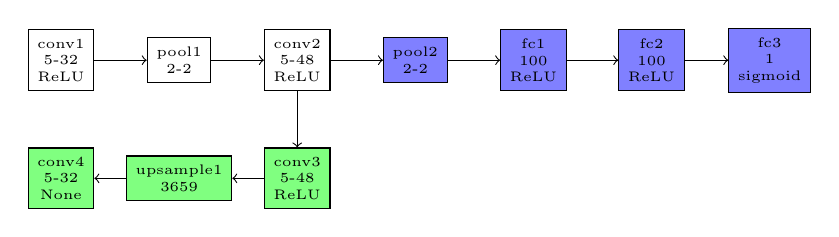
\begin{tikzpicture}[node distance=1.5cm]
	% encoder
	\node (conv1) [layer] {conv1\\5-32\\ReLU};
	\node (pool1) [layer,right of=conv1] {pool1\\2-2};
	\node (conv2) [layer,right of=pool1] {conv2\\5-48\\ReLU};
	% feature labelling
	\node (pool2) [layer,right of=conv2,fill=blue!50] {pool2\\2-2};
	\node (fc1) [layer,right of=pool2,fill=blue!50] {fc1\\100\\ReLU};
	\node (fc2) [layer,right of=fc1,fill=blue!50] {fc2\\100\\ReLU};
	\node (fc3) [layer,right of=fc2,fill=blue!50] {fc3\\1\\sigmoid};
	% decoder
	\node (conv3) [layer,below of=conv2,fill=green!50] {conv3\\5-48\\ReLU};
	\node (upsample1) [layer,left of=conv3,fill=green!50] {upsample1\\3659};
	\node (conv4) [layer,left of=upsample1,fill=green!50] {conv4\\5-32\\None};
	% connections
	\draw [->] (conv1) -- (pool1);
	\draw [->] (pool1) -- (conv2);
	\draw [->] (conv2) -- (pool2);
	\draw [->] (pool2) -- (fc1);
	\draw [->] (fc1) -- (fc2);
	\draw [->] (fc2) -- (fc3);
	\draw [->] (conv2) -- (conv3);
	\draw [->] (conv3) -- (upsample1);
	\draw [->] (upsample1) -- (conv4);
\end{tikzpicture}
}
\end{center}
\caption{Architectures}
\label{lenet_5}
\end{figure}

\section{Experiments with Deep DA}

Apply domain adaptation to the selected data.

\subsection{DDC: Deep Domain Confusion}

\subsection{DANN: Domain-Adversarial Neural Networks}

\subsection{DRCN: Deep Reconstruction-Classification Networks}

\section{Evaluation of Experiments}

Prepare visualisation of results.
